
\section{Details on the agent interface}

\label{app:interface}


Below is a showcase of how users could interact with the belief graph and clarifications in a hypothesised interface, to better iterate their inputs, to reach higher a quality and satisfaction of outputs. This is a crudely hypothesised, intentionally simple interface for the sake of research, but could be iterated and improved upon in many ways depending on application and users. 

\textbf{1. Default state}
On load of the app, there would be a text prompt input and space for output images, as is common across typical T2I interfaces. There would also be space for the user to view either clarifications from the model, or a graph interface, as part of the overall ``input'' section as these would act as a further input for future model output iterations. See \Cref{fig:interface1} below as reference. 

\begin{figure} [ht!]
    \centering
    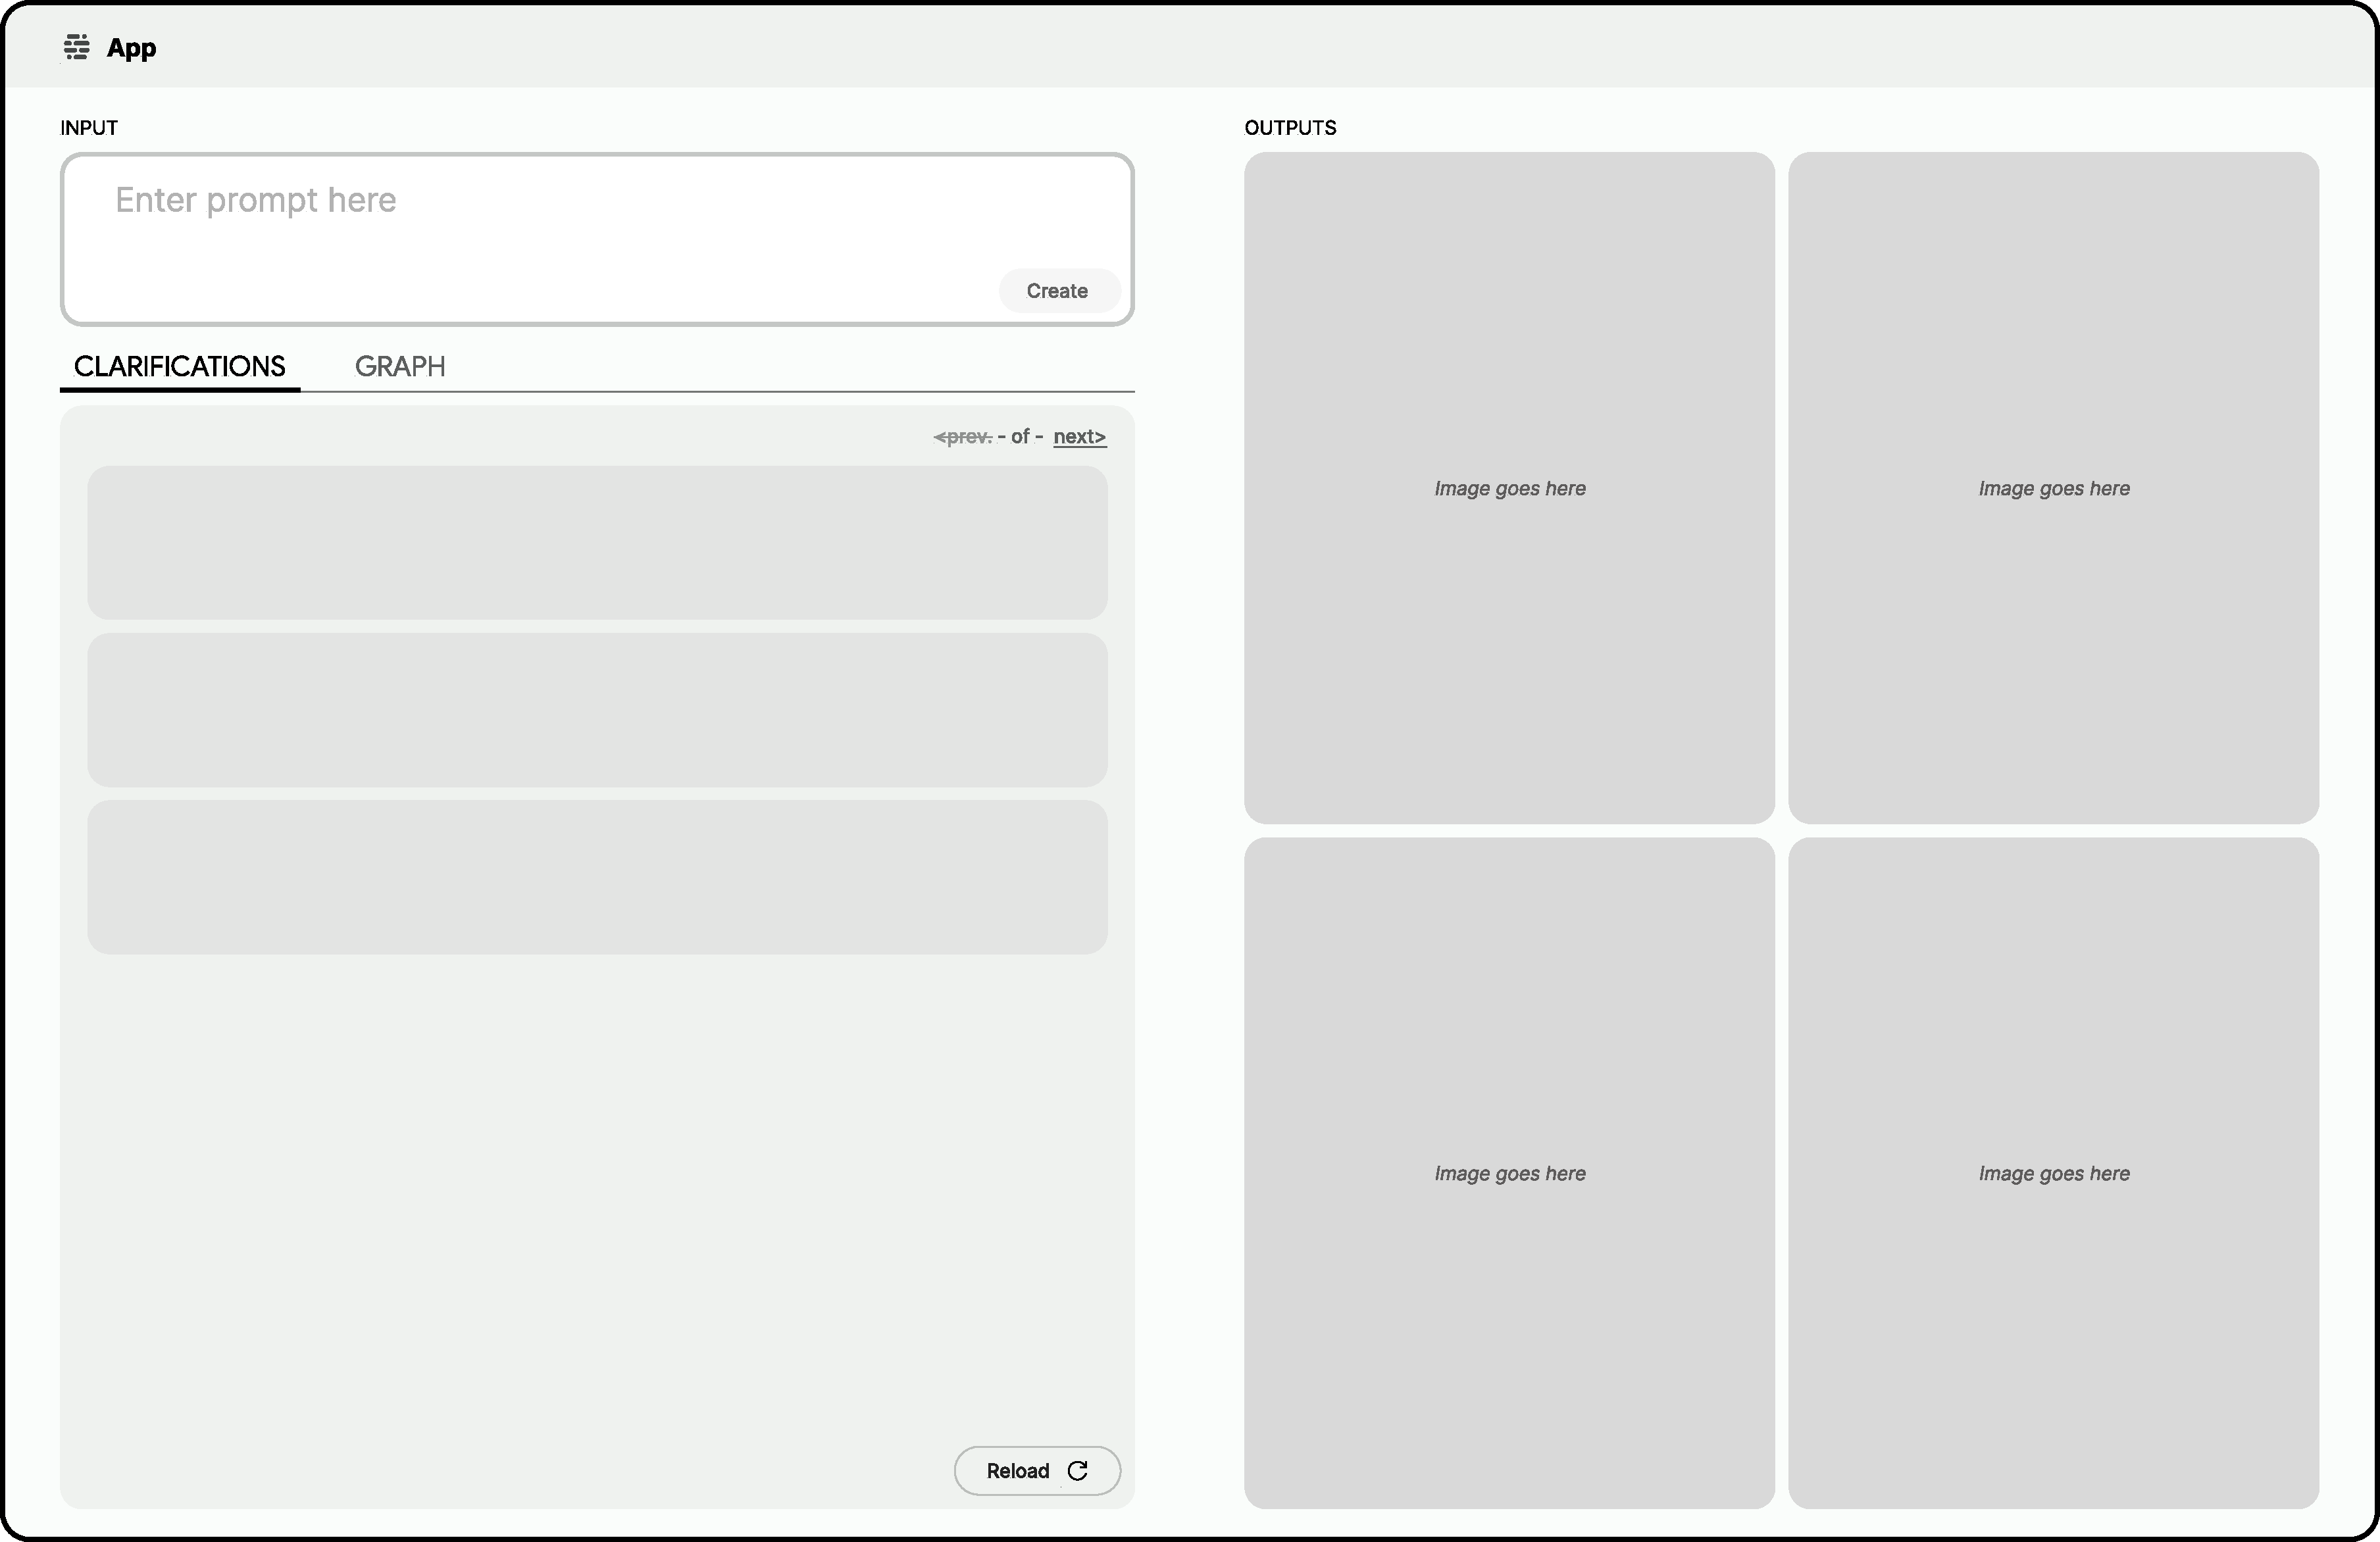
\includegraphics[width=.9\linewidth]{figures/Default.pdf}
    \caption{Default state of a possible interface.}
    \label{fig:interface1}
\end{figure} 

\textbf{2. Output images, with Clarifications} 
Once the user has submitted the prompt and the model has responded, there would be a set of images, as initial outputs from the users prompt. Below the input prompt would be a set of ``Clarifications'' in its populated state. These clarifications would ask the user specific questions that would be necessary to increase the specificity of the prompt, for the model to get a more accurate results aligned to the users intention, or to help the user realise their intention. Options would be given of the highest probability options for each Clarification, but the user could also fill in a totally new option via a free text field. Once answered by selection or text input, the clarifications would be added to the above, primary prompt for regeneration when the user selects. See \Cref{fig:interface2} below as reference.

\begin{figure} [ht!]
    \centering
    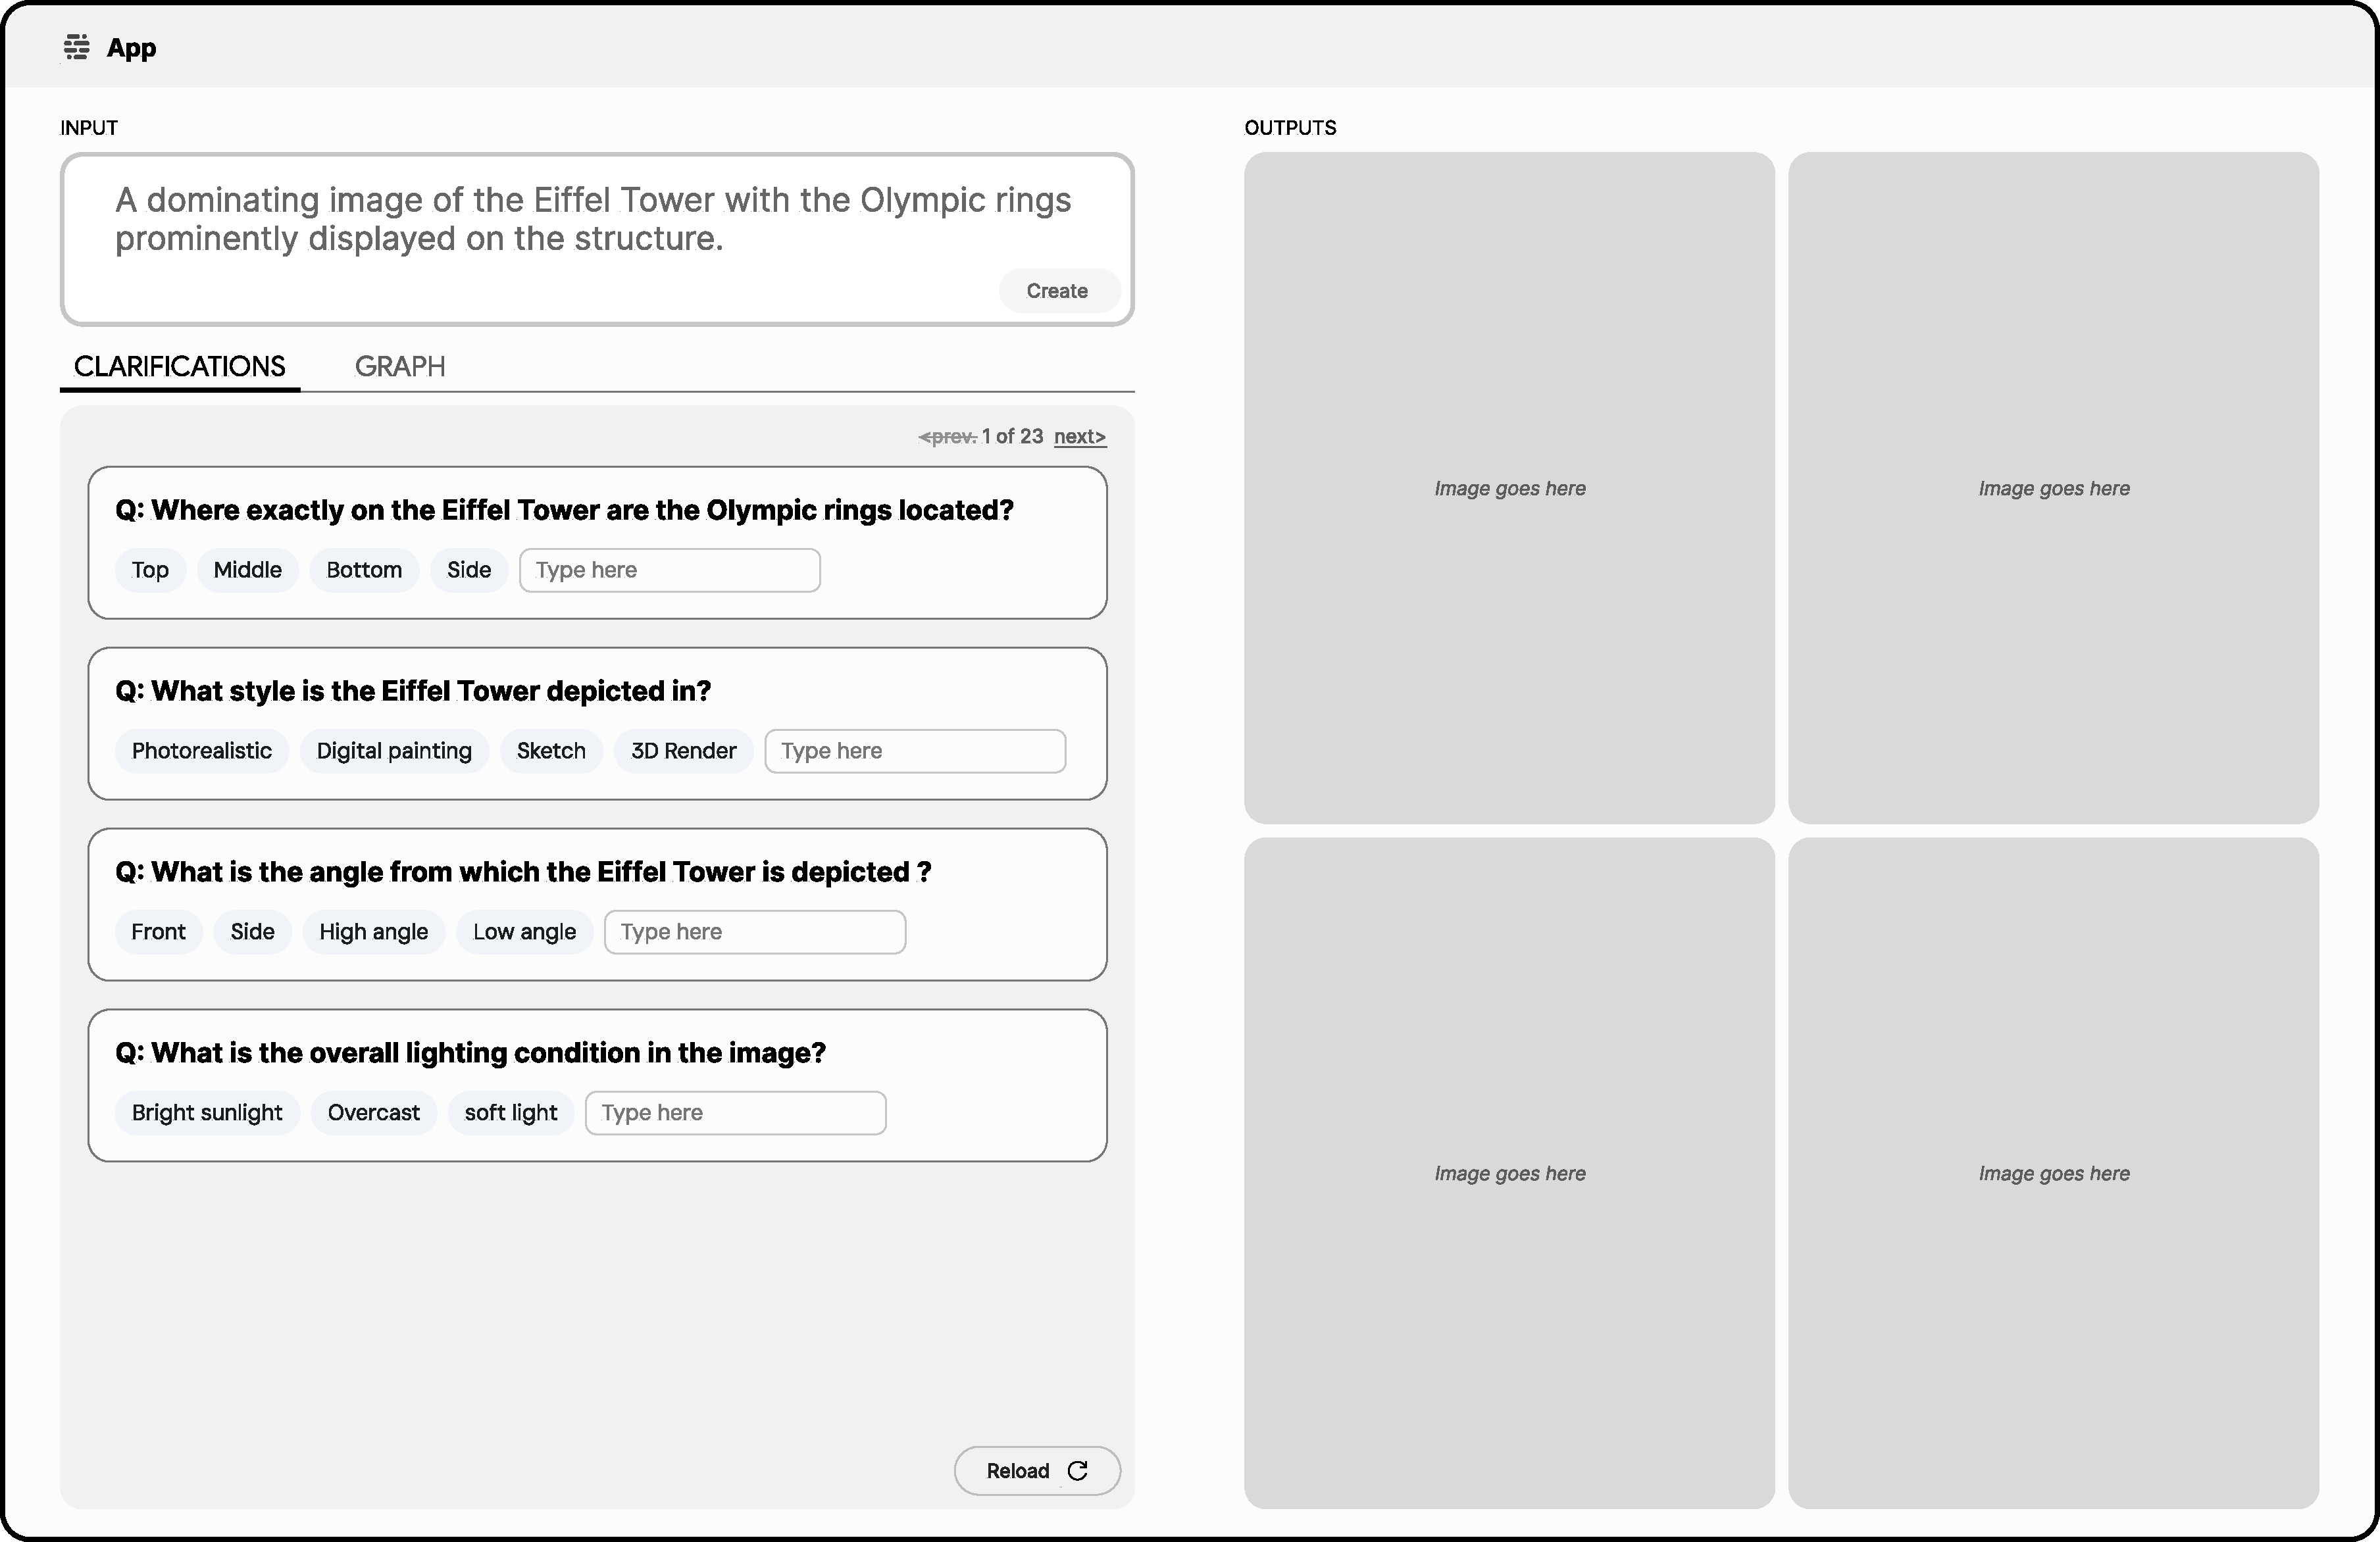
\includegraphics[width=.9\linewidth]{figures/Clarifications.pdf}
    \caption{Interface once prompt has been input with clarifications.}
    \label{fig:interface2}
\end{figure} 

\textbf{3. Graph Entities \& Attributes }
Instead of the clarifications, the user could select to instead view a Graph by clicking  Tab above the clarifications themselves. This graph would  be populated will all Entities from the prompt explicit and implicit visually defined differently (in this diagram by the dotted line surrounds implicit entities, but is a filled line when surrounding explicit entities). The graph layout will be structured, depicting relationships concentrically i.e. "on", "in" or "under" for example, will become child entities, and be displayed within the parent entities' boundary. For example a 'Mug' that has the relationship of 'on' a 'Table' entity, will sit within the boundary of 'Table', as also would a 'Plate' if that had the same child-parent relationship. 

Below the Graph would also be a list of 'cards' (i.e. boxed groups of information), one for each "explicit" or "implicit" entity. Within each card a user could see the status of implicit / explicit, and change this status to confirm or deny its presence. The user could also see a list of "attributes" associated to that entity, which the model has assumed. Each of these attributes could be changed by interacting with a list of alternatives via drop down. These lists are determined in terms of which items and order of items, based on the probability by which the model sees them, ordered with higest first. This probability would be made clear to the user to define the order by seeing the peercentage next to the label. See \Cref{fig:interface3} below as reference.

\begin{figure} [ht!]
    \centering
    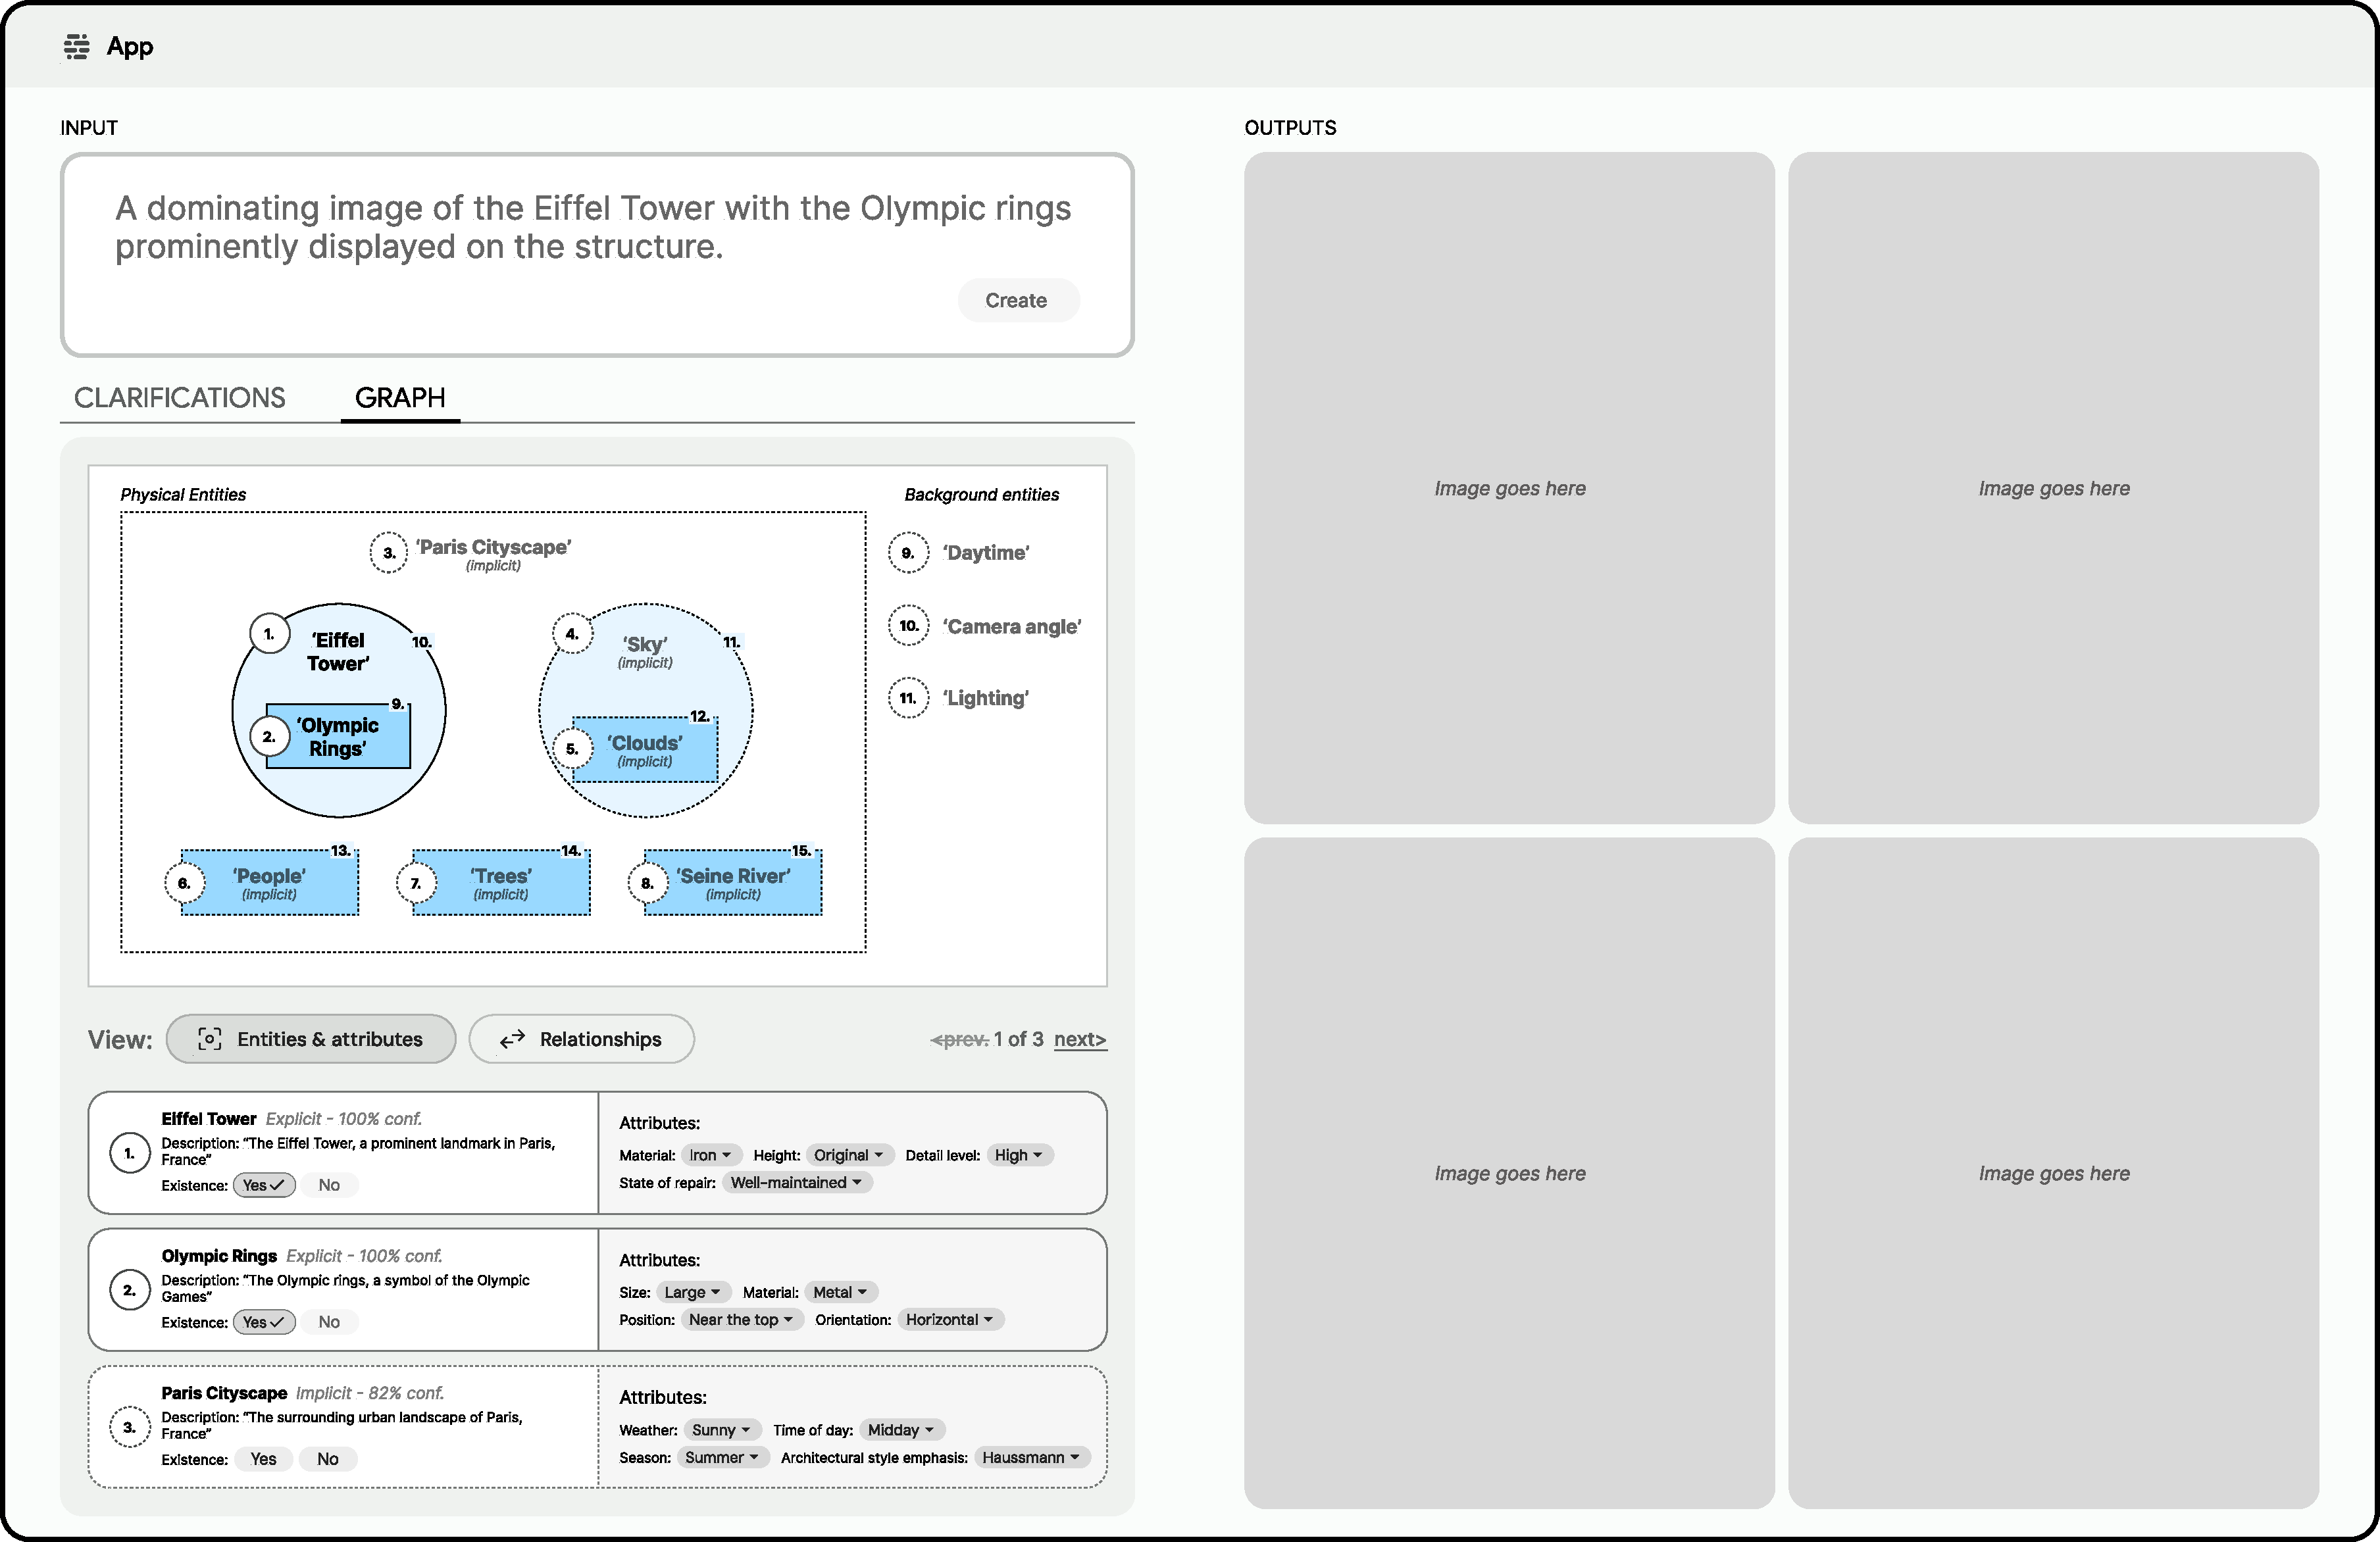
\includegraphics[width=.9\linewidth]{figures/Attributes.pdf}
    \caption{Interface with Graph displaying Entities, with cards below enabling a user to change attributes associated to each entity.}
    \label{fig:interface3}
\end{figure} 

\textbf{4. Graph Relationships} 
The user would also be able to change the state of the Graph and Cards, to instead focus on the relationships between entities, by toggling to "Relations". In this state the user would be able to focus on two specific entities (e.g. 'mug' and 'table'), see the description of the relationship (e.g. 'the mug is sitting on the table') and if desired change the relationship to an alternative (e.g. 'on', changed to 'under') via a drop down of options which the model determined as alternative options ordered by probability, as per attributes. See Figure \Cref{fig:interface4} below as reference.

\begin{figure} [ht!]
    \centering
    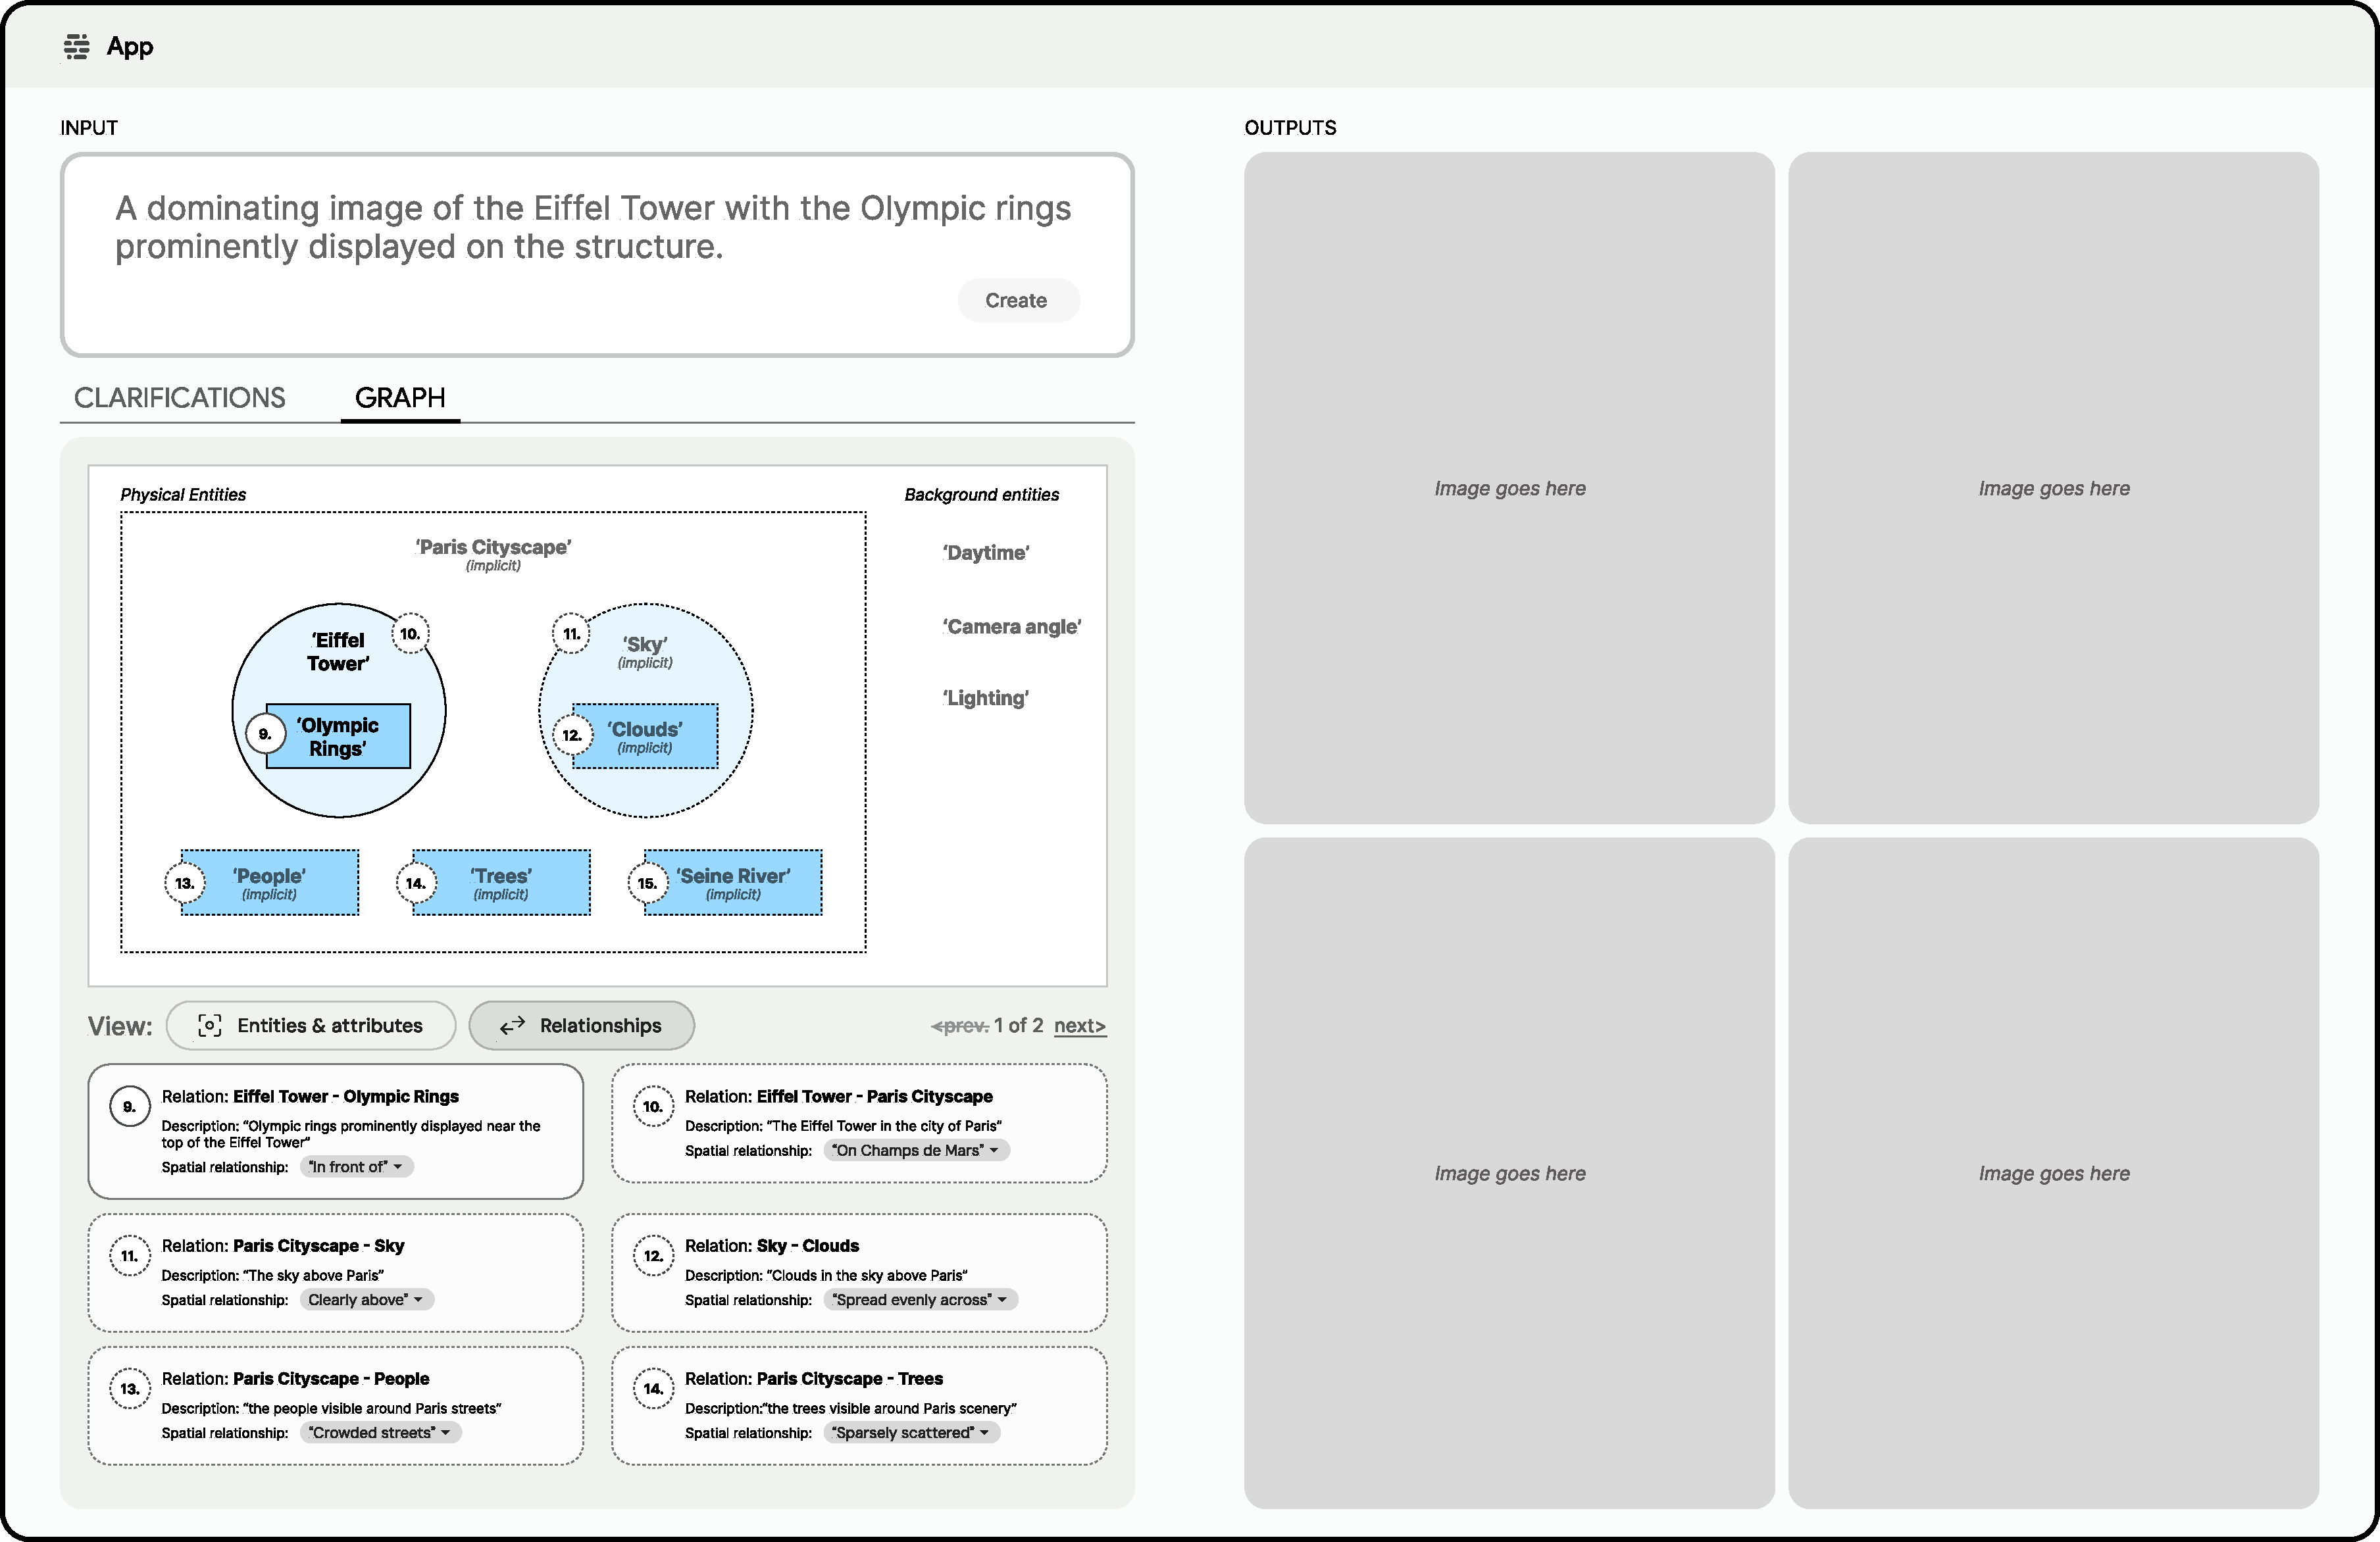
\includegraphics[width=.9\linewidth]{figures/Relations.pdf}
    \caption{Interface with Graph displaying relations between Entities, with cards below enabling a user to change relationships between entities.}
    \label{fig:interface4}
\end{figure} 

Once any of these changes are made the user could initiate a regeneration via the updated prompt to create a new set of output images, which can then be further refined via the same method. 

